\index{Renner, Britta}

\paragraph{Research Team}
Britta Renner (Professor), Youlia Spivak (Doctoral Fellow), Andries Oeberst (Doctoral Fellow), Martina Panzer (Doctoral Fellow).

 The Health Psychology Research Group is interested in the judgment and decision-making processes that underlie the onset, maintenance, and cessation of health-relevant behaviors with a particular emphasis on risk perception and reactions towards risk information. The activities of our research group are designed to further the synthesis of basic research on how people process and utilize health information and whether there are age-related differences in the functionality of health behavior changes. These efforts are motivated by the broader goal of developing theoretical frameworks that can be applied across a range of behavioral domains.

\null
\textbf{Research Highlights 2006}

 The DFG-funded longitudinal research project ``Risk Appraisal Consequences in Korea'' (RACK) is conducted in Seoul, South Korea, in collaboration with Prof. Dr. Ralf Schwarzer at the Free University of Berlin, Prof. Sunkyo Kwon at the Sookmyung University, Prof. Dr. Byung-Hwan Yang at the Hanyang University, and Prof. Dr. Ki-Chung Paik at the Dankook University (N = 1359). The research project focuses on the effects of individualized health feedback on health-related cognitions and health behavior changes in various age groups. This project is unique in its scope because for the first time the health behavior change process will be examined from a psychological perspective and can be compared directly to a western sample. See also http://www.gesundheitsrisiko.de/.

\newpage
\textit{Processing and Impact of Self-Relevant Risk Communication in Adulthood}

 At first glance, perceiving a health threat seems to be the most obvious prerequisite for the motivation to change risk behaviors. If one is not aware of the risky nature of one's actions, motivation for change cannot emerge. Therefore, a crucial barrier that health communication needs to overcome in order to be effective is to focus people's attention on information that pertains directly to their personal risk, thereby increasing the personal relevance of a health issue (Renner, Panzer, \& Oeberst, in press; Renner, Sch\"{u}z, \& Sniehotta, submitted; Renner \& Schwarzer, 2000, 2003; Renner \& Schupp, 2005; Weinstein, 1998, 2003). However, numerous empirical studies demonstrate differential acceptance of negative and positive risk information (cf. Croyle, Sun, \& Hart, 1997).

\enlargethispage*{0.5cm}

 Most researchers interpret these findings as evidence for motivated reasoning, arguing that people- who are informed that they have an elevated risk of disease minimize the seriousness of the health threat posed by the risk information and derogate the validity of the risk factor test in order to maintain a favorable sense of their health. However, the assumption of motivated reasoning has been challenged by the ``cue adaptive reasoning account'' (CARA; Renner, 2004). Extending the CARA research design introduced by Renner (2004), the present project focuses on the processing of self-relevant risk feedback (total cholesterol, blood pressure) in order to gain a more in-depth understanding of how people react towards risk communication. Moreover, the research project examines how reactions towards self-related risk feedback are related to age. This research is expected to provide particularly important information regarding effective risk communication. Analyses of spontaneous reactions toward blood pressure feedback show in accordance with the CARA approach that feedback valence and feedback expectedness are central processing categories.

\newpage
\textit{Health Cognitions and Health Behaviors}

 Engagement in preventive health behaviors is not merely determined by the awareness of objective health risks but it is mainly influenced by health beliefs and specific health cognitions (Renner \& Schwarzer, 2003, 2005). The goal of the research project based on data from the ``Risk Appraisal Consequences in Korea'' (RACK) and Berlin Risk Appraisal and Health Motivation Study (BRAHMS) is to further the development of current health models, in particular the Health Action Process Approach (HAPA; Renner \& Schwarzer, 2003; 2005; Renner, Yang, Paik, Kim, Roh, Song, \& Schwarzer, in press; Schwarzer, 1999; Schwarzer \& Fuchs, 1996). HAPA is regarded as a heuristic to better understand the complex mechanisms that operate when people become motivated to change their behavior, and when they attempt to resist temptations. It applies to all health-compromising and health-enhancing behaviors and pays particular attention to postintentional mechanisms, and it conveys an explicit self-regulation perspective. Four areas of health behavior are the focus of the study: Nutrition, physical activity, smoking, and alcohol consumption. First results for nutrition confirm the predictive power of the Health Action Process Approach but point to the role of gender in the self-regulation of dietary behaviors (Renner et al., in press; see Figure \ref{fig2:profBrittaRenner}).

\begin{figure}[h!tb]
  \begin{center}
    \resizebox{0.5\textwidth}{!}{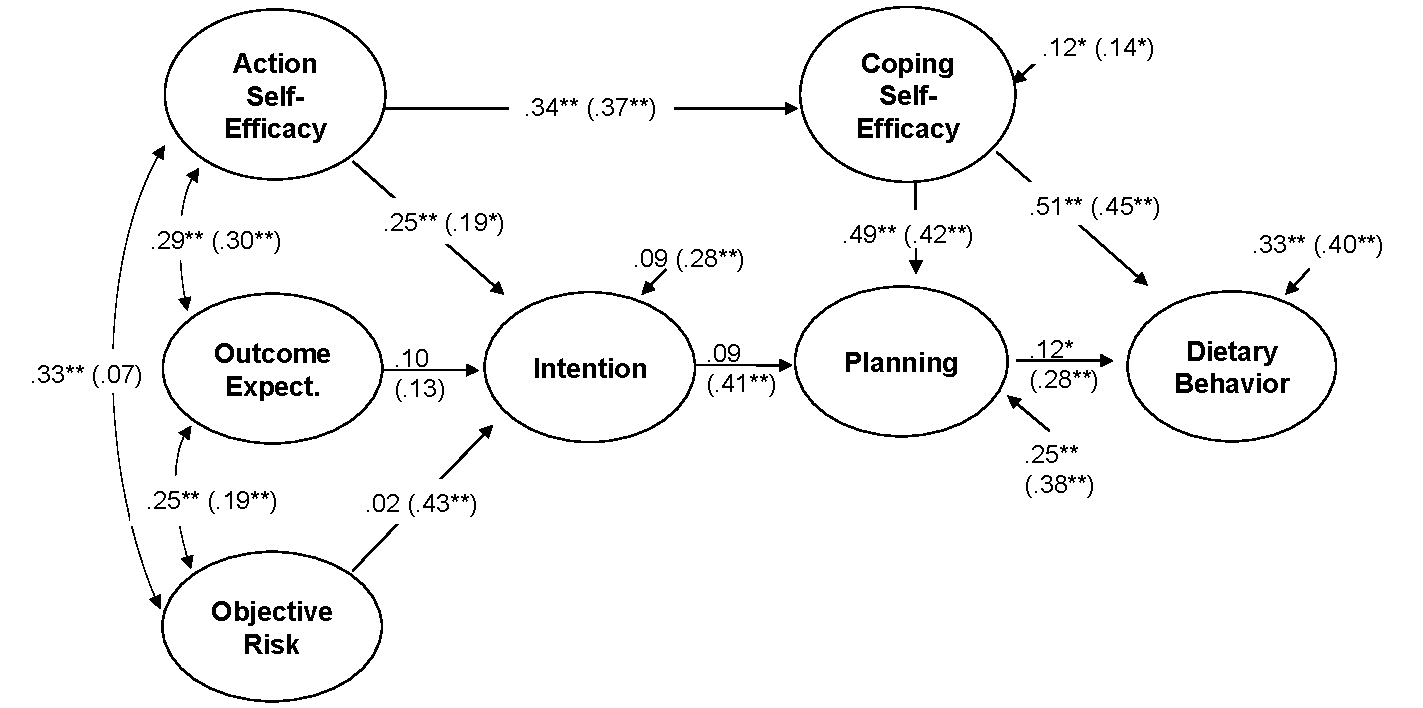
\includegraphics{profBrittaRenner-fig2}}
    \caption{Two-group prediction model for dietary behaviors in South Korean men and women. Coefficients for women in parentheses. (Renner et al., in press.)}
    \label{fig2:profBrittaRenner}
  \end{center}
\end{figure}


\newpage
 To date, little is known about how determinants of the process of health behavior change vary across the lifespan. Social cognition models of health behavior are commonly understood as being universal, implying that they are applicable to groups that vary, for example, in age or cultural background. Cultural uniqueness and specific characteristics of lifespan development, however, necessitate the study of differential effects. For instance, previous research suggests that with increasing age, risk perception becomes a more important motivational drive even though the actual health status may have not changed (Renner, Knoll, \& Schwarzer, 2000; Schwarzer \& Renner, 2000).

 Therefore, the present research project also examines whether there are age-related differences in health-related cognitions, health behaviors, and the functionality of health behavior changes. These efforts are motivated by the broader goal of developing theoretical frameworks that can be applied across a range of behavioral domains.

 Accordingly, the Health Action Process Approach is examined in younger and middle-aged/older adults from South-Korea who participated in a longitudinal health screening study with a 6-month time lag. First results suggest a different motivation for the involvement in physical activity as a function of age (Renner, Spivak, Kwon, \& Schwarzer, submitted).

{\textit{Health-Related Behavior, Risk Perception, \& Risk Stereotypes}

 Extending previous research, this research project examines not only what people consider as risky (high risk stereotype) but also what they consider as safe (low risk stereotype). This approach allows testing the hypothesis that it is the ratio of the low risk stereotype, the self, and the high risk stereotype which determine risk perception (Renner \& Schwarzer, 2003; Renner \& Schupp, 2005). Part of the research program examines whether low and high risk stereotype images are related to risk perceptions and, in particular, to unrealistic optimism. Particularly, we investigate whether people actively construe images of low and high risk stereotypes in order to maintain a favourable standing in comparison to others.

 The second goal of this project which is conducted in cooperation with the University of Konstanz and funded by the DFG is to examine the effects of risk stereotypes and of affect on risk perceptions in the domain of HIV and sexually transmitted diseases. This research project incorporates four new aspects: (1) devising a new method to assess self-related risk perceptions which enables identifying unrealistically optimistic risk perceptions at the individual rather than at the group level; (2) examining the role of stereotypical beliefs about persons that are high or low at risk (risk stereotypes) for self-related risk perceptions; (3) examining the role of affect for other-related risk perception from a multi-system perspective including established neuroimaging and psychophysiological measures; and (4) assessing the interplay of self-related and other-related risk perceptions. Exploring these issues is considered relevant for a better understanding of the knowledge-behavior gap, i.e. the comparably low prevalence of protective behavior despite high knowledge about health risks. In the long run, this research will contribute towards the overarching goal of devising more effective risk interventions called for by the World Health Organization and other health expert institutions.


\paragraph{Collaborations}
\begin{itemize}
\item Free University of Berlin \\ Prof. Dr. Ralf Schwarzer 
\item Sookmyung University, South Korea \\ Prof. Dr. Sunkyo Kwon
\item Hanyang University, South Korea \\ Prof. Dr. Byung-Hwan Yang
\item Dankook University, South Korea \\ Prof. Dr. Ki-Chung Paik
\item University of Konstanz \\ Prof. Dr. Harald Schupp 
\item KTL Public Health Institute Helsinki \\ Dr. Pilvikki Absetz
\item Charit\'e Berlin \\ Prof. Dr. Claudia Spies; Dr. Birte Dohnke; Dr. Edith Weiss-Gerlach; Dr. Andrea Mossner
\item Universidad Estatal a Distancia San Jos\'e \\Dr. Benicio Guti\'errez-Do\~na
\end{itemize}

\begin{bibunit}[apalike]
\nocite{*}
\putbib[profBrittaRenner1]
\end{bibunit}


\paragraph{Grants}
\begin{itemize}
\item DFG Re1583/2-1 (PI: B. Renner in cooperation with R. Schwarzer, Free University Berlin): Individualized Feedback after Blood Pressure and Cholesterol Screenings: The Role of Health Beliefs, Health Behaviors, and Actual Health Status.  
\item DFG RE 1583/3-1  (PI: B. Renner in cooperation with H. Schupp, University of Konstanz): Self-Related and Other-Related Risk Perception: The Impact of Risk Stereotypes and Affective Responses.
\item CONARE-Project, Costa Rica S. No26-06, 01/08/06 (Start: 2007). (PI: B. Renner in cooperation with B. Guti\'errez-Do\~na, Universidad Estatal a Distancia San Jos\'e and R. Schwarzer, Free University Berlin): Individualized Feedback after Blood Pressure and Cholesterol Screenings. 

\item BMBF (PI: JCLL). B. Renner: subproject ``Health Promotion'' within the joint research project ``Effects of Matches/Mismatches between Aspects of Human and Social Capital, Corporate Strategy and Work Organization on the Physical and Mental Well-Being of Employees''. 
\end{itemize}
